\chapter[Processo de Engenharia de Requisitos]{Processo de Engenharia de Requisitos}\label{cap4}

Esse processo foi desenhado utilizando ferramenta ``\textit{BIZAGI modeler}''. Houveram 5 evoluções,
presentes no apêndice \ref{apendice:evolution}, a partir do primeiro esboço até chegar a versão apresentada na imagem \ref{fig:processo}.

Como foi descrito no capítulo \ref{cap3} o processo criado foi estruturado baseando-se no
SAFe mantendo os três níveis estruturais do framework, portifólio, programa e time
que estão detalhados na sessão \ref{safe}.

A manutenção da rastreabilidade dos requisitos, tem papel fundamental para a criação deste processo,
entretando no processo SAFe não há a definição plena da manutenbilidade da rastreabilidade entre os
vários níveis. Portanto há a necessidade de criação de uma adaptação, para isso utiliza-se de
outro processo base, o RUP.

É fundamental destacar que o problema da escolha de um abordagem não esta em considerar
a mutabilidade dos requisitos e sim em como tratar essas mudanças que são inevitáveis.
Pensando nisso foram adicionadas atividades de gerência de mudanças baseadas no RUP,
para sanar um possível risco na comunicação e gerência do projeto devido a não experiência
de trabalho entre os membros do grupo. Esse processo ocorre de forma eventual e paralela
e será detalhado na sessão \ref{sec:gerencia}.

[Papeis]
[Artefatos]
[Atividades]

\begin{figure}[H]
    \centering
	\includegraphics[keepaspectratio=true,scale=0.5]{figuras/Processo_05.eps}
    \caption{Visão geral do processo desenvolvido para o projeto.}
    \label{fig:processo}
\end{figure}

\section{Scaled Agile Framework}\label{safe}

Nessa sessão serão descritos os níveis que compoem o SAFe(Portifólio, Programa e Time).
Sendo mostrado o objetivo cada nível como também as atividades que a compoem.

\subsection{Portifólio}

No processo criado nesse trabalho, esse nível tem como objetivo levantar e estabelecer
uma abstração de alto nível dos requisitos do negócio. Esse levantamento ocorrerá
por meio da efetuação das atividades Entender Contexto do Cliente e Levantar Épicos
e Revisar e Analisar. As técnicas utilizadas para a execução de cada atividade serão
a análise documental, workshops e Brainstorms.

\subsubsection{Processo}

\begin{figure}[H]
    \centering
  \includegraphics[keepaspectratio=true,scale=0.5]{figuras/portifa.eps}
    \caption{Visão geral do nível de portifólio.}
    \label{fig:portifa}
\end{figure}

\subsubsection{Papéis}

\textbf{Gerente de Portfólio}: Possui a mais alto nível de decisão do processo, buscam compreender
a estratégia da empresa, tecnologia e restrições. No nosso contexto ele terá também
a função de Dono do Épico, que é responsável pela condução dos épicos para identificação
através da análise do processo e do sistema Kanban. Quando aceito para implementação,
trabalha com a equipe de desenvolvimento e de gestão de produtos para iniciar as atividades
de desenvolvimento necessárias para contemplar o épico.

\subsubsection{Artefatos}



\begin{description}
  \item[A - Processo do cliente:]
  Artefato de entrada que será fornecido pelo cliente ao Gerente de portifólio.
  Contém o processo otimizado, da organização do cliente, modelado na notação BPMN.\cite{BPMN}
  \item [B - Contexto do cliente]
  Artefato fornecido pelo cliente, que descreve resumidamente o contexto do problema
  a ser solucionado e uma síntese do motivo da contratação para o desenvolvimento de software.
  \item [C - Tema de investimento: ]
  Representa os objetivos do financiamento da solução, área que irá atuar e valores da empresa.
  É representado por uma pequena proposição com uma breve descrição. É o requisito de
  mais alto nível no processo. Compoem o portifolio backlog.\cite{themes}
  \item [D - Lista de Épicos:]
  Os épicos representam uma iniciativa de negócio, pode ser algo que gere alto valor
  para o cliente ou alto valor para o desenvolvimento de software, como inovações de arquitetura.
  É um requisito ainda de alto nível e deve ser sempre coletado, analisado e refinado.
  Possui três níveis de dimensão
    \begin{enumerate}
      \item \textbf{Tempo: } A implementação pode levar muitas iterações e releases.
      \item \textbf{Escopo: } Afeta vários níveis no projeto, por ser alto nível a mudança
      de um épico pode ocasionar um grande impacto e custar muito para a organização.
      \item \textbf{Negócio: } Afeta vários departamentos na área de negócios, representa
      a entrega de valor direta para o cliente no portifólio.
    \end{enumerate}
  A lista de épicos é o resultado de um brainstorm de possíveis épicos para serem entregues,
  que passarão depois por uma atividade para filtrar e analisar a consistensia dos mesmos.
  \item [E - Backlog do Portifólio]
  Backlog de Portifólio: É uma pilha que contem os épicos detalhados e organizados
  por ordem de prioridade de implementação. É feito uma estimativa em pontuações
  que representam a complexidade do épico. Para fazer essa estimativa o épico deve
  ser detalhado para facilitar a identificação de possível divisão desse épico em
  outros épicos, e a análise da consistência do mesmo.\cite{epics}

  Para estimar o valor do épico, pode ser utilizado o template no anexo \ref{apendice:templates}
\end{description}

\subsubsection{Atividades}

  \begin{table}[H]
    \centering
      \begin{tabular}{| m{5em} | m{10cm} |}
        \hline
        ID       & 01   \\ \hline
        Nome     & Entender Contexto do Cliente   \\ \hline
        Objetivo & Serão realizadas reuniões entre o cliente e o gerente de portifólio para um primeiro contato com o objetivo de entender e esclarecer o contexto do problema. \\ \hline
        Entradas & Processo do Cliente, Contexto do Cliente.   \\ \hline
        Saídas   & Tema de Ivestimento. \\ \hline
        Papel Responsável   & Gerente de Portfólio. \\ \hline
      \end{tabular}
      \caption{Legenda da Tabela}
      \label{tabela:atividade1}
  \end{table}

  \begin{table}[H]
    \centering
      \begin{tabular}{| m{5em} | m{10cm} |}
        \hline
        ID       & 02   \\ \hline
        Nome     & Levantar Épicos   \\ \hline
        Objetivo & Brainstorm de ideias relacionadas ao tema de investimento e escrita de épicos. \\ \hline
        Entradas & Tema de Investimento   \\ \hline
        Saídas   & Lista de Épicos \\ \hline
        Papel Responsável   & Gerente de Portfólio. \\ \hline
      \end{tabular}
      \caption{Legenda da Tabela}
      \label{tabela:atividade2}
  \end{table}

  \begin{table}[H]
    \centering
      \begin{tabular}{| m{5em} | m{10cm} |}
        \hline
        ID       & 03   \\ \hline
        Nome     & Revisar e Analisar   \\ \hline
        Objetivo & Os épicos levantados são detalhados, analisados e revisados. Algumas features podem surgir e irão compor a versão inicial do Backlog do Programa. \\ \hline
        Entradas & Lista de Épicos   \\ \hline
        Saídas   & Backlog do Programa, Backlog do Portifólio(Atualizado). \\ \hline
        Papel Responsável   & Gerente de Portfólio. \\ \hline
      \end{tabular}
      \caption{Legenda da Tabela}
      \label{tabela:atividade3}
  \end{table}

  \subsection{Programa}

  Nesse nível do processo, foram definidas as atividades Levantas Requistos não funcionais,
  Selecionar Épicos para a Iteração, Levantar Features, Levantar Histórias de Usuário e Planejar Releases.
  Este etapa conscite em indentificar requisitos palpáveis e a partir disso estabelecer estratégias
  juntamente com o nível de time para a implementação da solução de software.

  \subsubsection{Processo}

  \begin{figure}[H]
      \centering
    \includegraphics[keepaspectratio=true,scale=0.5]{figuras/programa.eps}
      \caption{Visão geral do nível de programa.}
      \label{fig:progama}
  \end{figure}

  \subsubsection{Papéis}

    \textbf{Gerente do Produto}: Responsável por definir e priorizar o backlog de programa.
    Além de ser responsável pela construção, manutenção e apresentação da Visão e Roadmap
    e gerenciar o conteúdo da realease.

  \subsubsection{Artefatos}

  \begin{description}
    \item[A - Visão]
    O visão representa um descrição da soluçã a ser desenvolvida , baseade nas necessidades
    dos stakeholders. Contem uma coleção inicial de features , requisitos não funcionais,
    regras , padrões que devem ser seguidos , e restrições do projeto. Contem uma sintese dos
    objetivos a serem atingidos no programa e servirá de base para os seguintes níveis.\cite{vision}
    \item[B - Épico da Iteração]
    É apenas a representação do épico do backlog de portifólio que foi selecionado
    para passar pela a iteração de detalhamento e especificação.
    \item[C - Roadmap]
    O roadmap estabilisa e comunica e alinha a interação entre o nível de time e programa,
    tem o objetivo de demonstrar de forma transparente, natural e em alto nível, as entregas
    em uma linha do tempo. Geralmente representa de 3 a 6 meses de planejamento, composto objetivos
    e o que será desenvolvido em cada release. A previsão é gerada de forma balanceada e cuidadosa,
    para evitar possíveis retrabalhos. \cite{roadmap}
    \item[D - Backlog do Programa]
    Mantém em um único lugar as funcionalidades que deverão ser desenvolvidas nas releases
    e que entrarão no ágile release train. É considerada a chave do sucesso para economia
    do nível de programa. Um backlog bem organizado diminui os atrazos e o custo do desenvolvimento.
    É utilizado como base para gerar o roadmap e como a base do nível de time\cite{programbacklog}.
    A priorização das features são realizadas utilizando a prática de o trabalho mais pesado e
    mais curto vem primeiro. Para medir o peso do trabalho é utilizada a formula da imagem abaixo  e também
    uma tabela de comparação modelo presente no anexo X\cite{wsjf}.

    \begin{figure}[H]
        \centering
      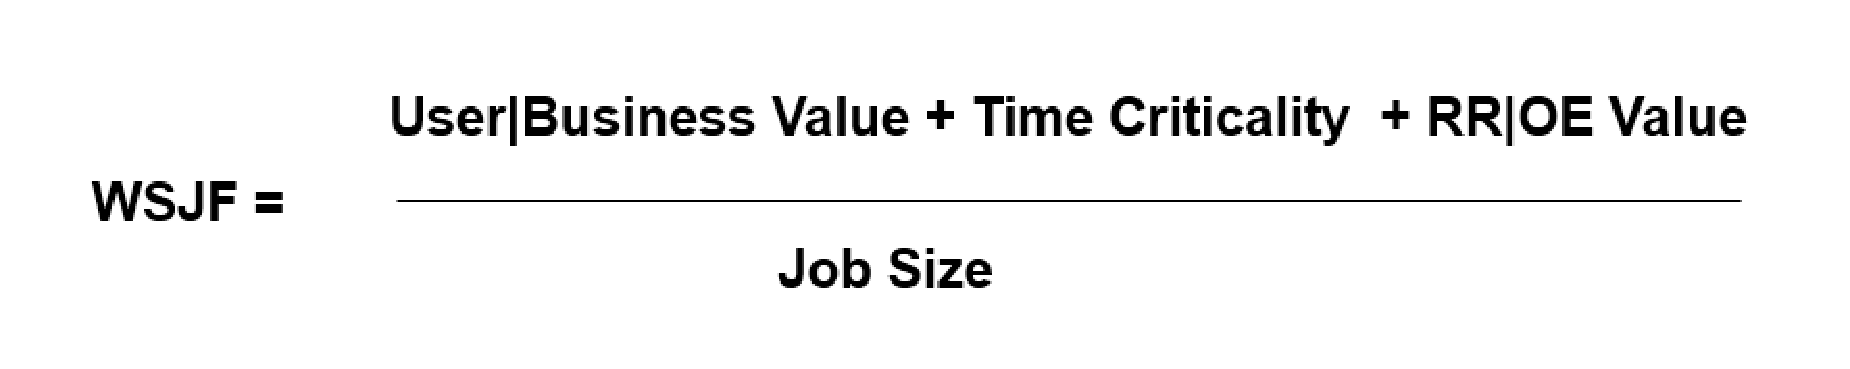
\includegraphics[keepaspectratio=true,scale=0.3]{figuras/WSJF-Formula.eps}
        \caption{Fómula do cálculo do valor de uma feature.}
        \label{fig:wsjf}
    \end{figure}


  \end{description}


  \subsubsection{Atividades}

  \begin{table}[H]
    \centering
      \begin{tabular}{| m{5em} | m{10cm} |}
        \hline
        ID       & 04   \\ \hline
        Nome     & Levantar Requisitos Não Funcionais   \\ \hline
        Objetivo & Serão realizadas reuniões entre o cliente e o time. Serão levantas as melhores condições para a solução. Ex: Tecnologia, Plataforma, Usabilidade. Também serão levantadas as restrições e padrões que o projeto deve seguir. \\ \hline
        Entradas & Backlog do Programa e Backlog do Portifólio.   \\ \hline
        Saídas   & Visão \\ \hline
        Papel Responsável   & Gerente de Programa. \\ \hline
      \end{tabular}
      \caption{Legenda da Tabela}
      \label{tabela:atividade4}
  \end{table}

  \begin{table}[H]
    \centering
      \begin{tabular}{| m{5em} | m{10cm} |}
        \hline
        ID       & 05   \\ \hline
        Nome     & Selecionar Épico para Iteração   \\ \hline
        Objetivo & Atividade de priorização dos épicos, onde serão selecionados os épicos a serem abordados na iteração de acordo com o backlog do portifólio. \\ \hline
        Entradas & Backlog do Portifólio.\\ \hline
        Saídas   & Épico da iteração \\ \hline
        Papel Responsável   & Gerente de Programa. \\ \hline
      \end{tabular}
      \caption{Legenda da Tabela}
      \label{tabela:atividade5}
  \end{table}

  \begin{table}[H]
    \centering
      \begin{tabular}{| m{5em} | m{10cm} |}
        \hline
        ID       & 06   \\ \hline
        Nome     & Levantar de Features   \\ \hline
        Objetivo & Atividade para levantar detalhadamente as features que estão relacionadas aos épicos selecionados. \\ \hline
        Entradas & Épico da Iteração\\ \hline
        Saídas   & Backlog do Programa \\ \hline
        Papel Responsável   & Gerente de Programa. \\ \hline
      \end{tabular}
      \caption{Legenda da Tabela}
      \label{tabela:atividade6}
  \end{table}

  \begin{table}[H]
    \centering
      \begin{tabular}{| m{5em} | m{10cm} |}
        \hline
        ID       & 07   \\ \hline
        Nome     & Levatar Histórias  \\ \hline
        Objetivo & Atividade para levantar histórias de usuários, relacionadas as features levantadas, em alto nível, sem detalhamentos.  \\ \hline
        Entradas & Backlog do Programa\\ \hline
        Saídas   & Backlog do Time \\ \hline
        Papel Responsável   & Gerente de Programa. \\ \hline
      \end{tabular}
      \caption{Legenda da Tabela}
      \label{tabela:atividade7}
  \end{table}

  \begin{table}[H]
    \centering
      \begin{tabular}{| m{5em} | m{10cm} |}
        \hline
        ID       & 08   \\ \hline
        Nome     & Planejar Releases  \\ \hline
        Objetivo & Atividade para planejar as releases da iteração, irá gerá o roadmap e o program backlog com as features priorizadas e organizada em uma linha do tempo de entregas. São definidos os objetivos de cada release também. \\ \hline
        Entradas & Backlog do Time, Backlog do Programa. \\ \hline
        Saídas   & Backlog do Programa, RoadMap \\ \hline
        Papel Responsável   & Gerente de Programa. \\ \hline
      \end{tabular}
      \caption{Legenda da Tabela}
      \label{tabela:atividade8}
  \end{table}

\subsection{Time}
  \subsubsection{Processo}

  \begin{figure}[H]
      \centering
    \includegraphics[keepaspectratio=true,scale=0.5]{figuras/time.eps}
      \caption{Visão geral do nível de time.}
      \label{fig:time}
  \end{figure}

  \subsubsection{Papéis}

\textbf{Dono do Produto}: Responsável por definir, manter e priorizar o backlog do time,
elaborar e validade as histórias de usuário, participar do planejamento e validação
da Sprint de tal modo a agilizar a execução de programas prioritários, mantendo a
integridade conceitual e técnica dos recursos ou componentes do time. Possui um papel
significativo no que se diz respeito a qualidade.

\textbf{Scrum Master}: Responsável por facilitar as interações da equipe e ajuda
a dirigir os esforços da equipe para a melhora continua.

\textbf{Team}: São os indivíduos capazes de definir, construir e testar em uma interação
de curto tempo. Inclui desenvolvedores, testadores, um Scrum Master e Dono do Produto.

  \subsubsection{Artefatos}

\begin{description}
  \item[A - Backlog do Time]
  Tem como conteúdo, basicamente todas as coisa que o time deve fazer para gerar
  os pacotes de software e entregar valor para o cliente. É composto por histórias
  de usuário, histórias técnicas, defeitos, necessidades de infraestrutura, necessidades
  do time, refatoração, e qualquer outra coisa que o time precisa fazer. Muitas entidades
  contribuem para a geração do backlog do time como representado na imagem abaixo:

  \begin{figure}[H]
      \centering
    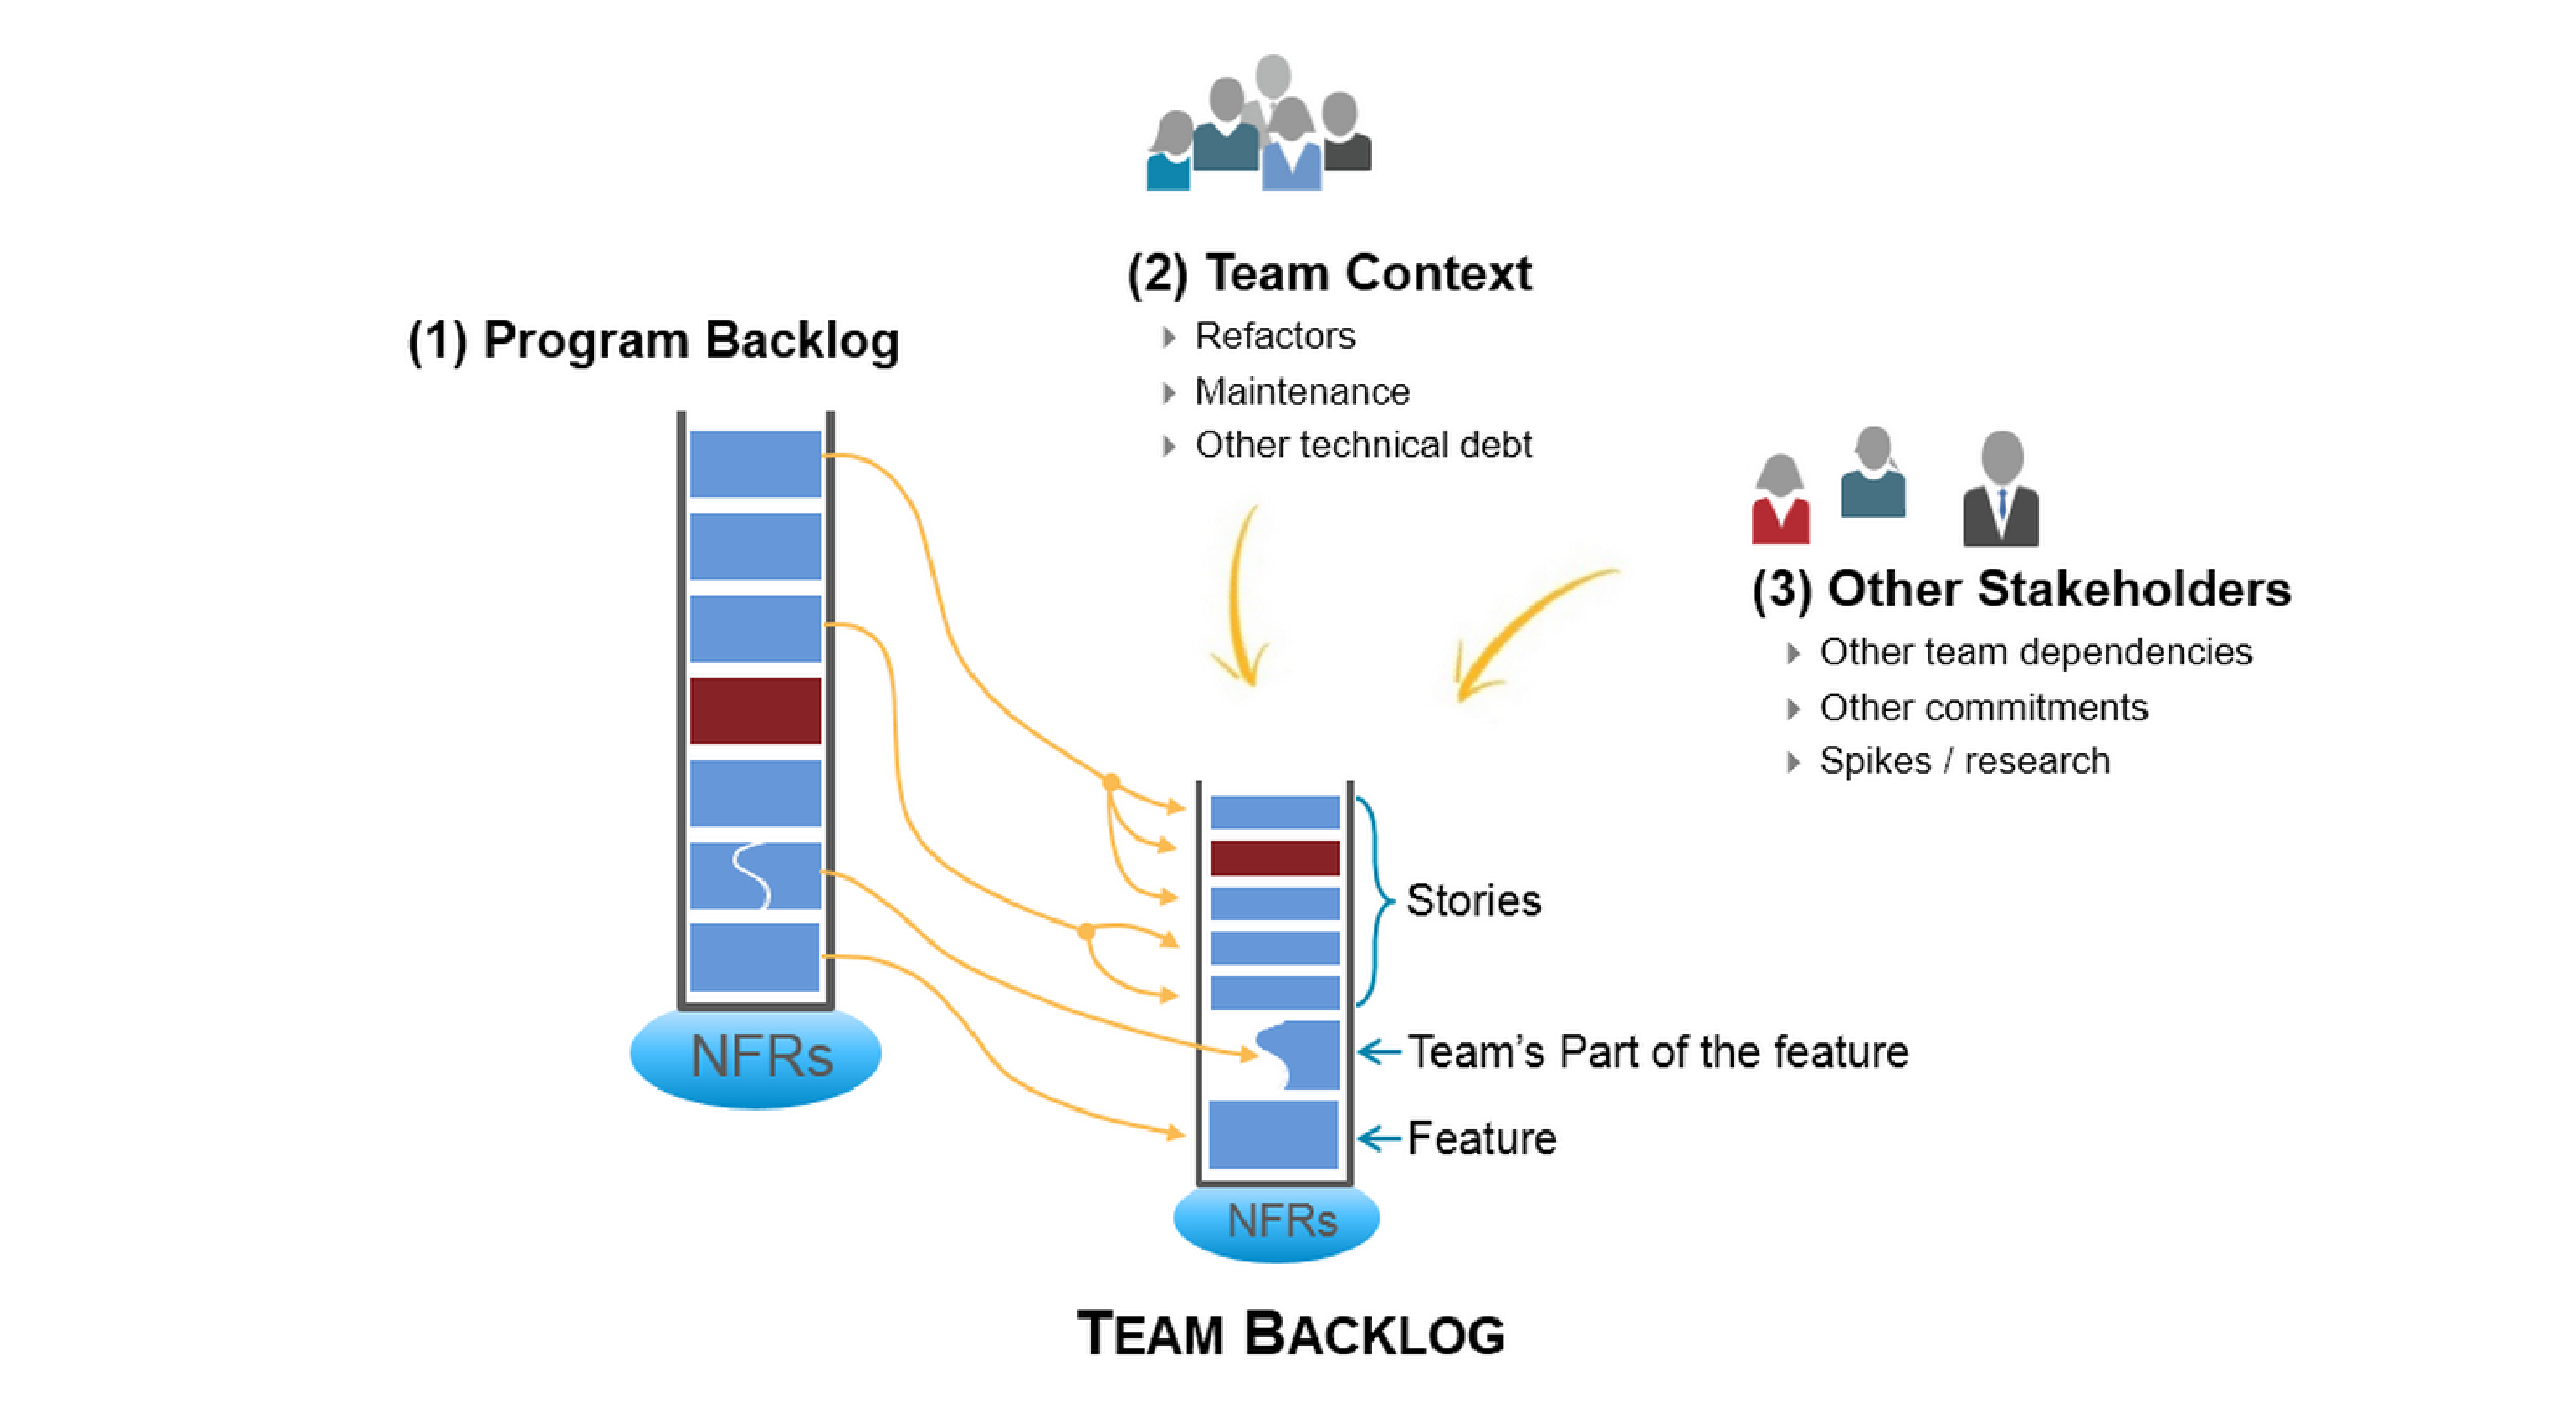
\includegraphics[keepaspectratio=true,scale=0.3]{figuras/TeamBacklog.eps}
      \caption{Estruturação do backlog do time.}
      \label{fig:backlog}
  \end{figure}

  Nota-se que na criação do backlog de time as features são ramificadas em pequenas histórias.


  \item[B - Lista de melhorias e Correções]
   E gerada para registrar evoluções nos artefatos que foram obtidas através de feedbacks
  de algum artefato já entregue. Presente em vários níveis.

\end{description}


  \subsubsection{Atividades}

  \begin{table}[H]
    \centering
      \begin{tabular}{| m{5em} | m{10cm} |}
        \hline
        ID       & 09   \\ \hline
        Nome     & Detalhar Histórias de Usuário  \\ \hline
        Objetivo & Serão detalhados as histórias relativas as feature corrente, como principal objetivo definir os critériaos de aceitação para teste das mesmas.  \\ \hline
        Entradas & Roadmap, Backlog do Time\\ \hline
        Saídas   & Backlog do Time (Refinado) \\ \hline
        Papel Responsável   & Gerente de Produto. \\ \hline
      \end{tabular}
      \caption{Legenda da Tabela}
      \label{tabela:atividade9}
  \end{table}

  \begin{table}[H]
    \centering
      \begin{tabular}{| m{5em} | m{10cm} |}
        \hline
        ID       & 10   \\ \hline
        Nome     & Levantar e Priorizar Necessidades do Time  \\ \hline
        Objetivo & Serão identificados os spikes, necessidades que o time precisa suprir durante a sprint, para evoluir.  \\ \hline
        Entradas & Backlog do Time (Refinado)\\ \hline
        Saídas   & Backlog do Time (Refinado) \\ \hline
        Papel Responsável   & Gerente de Produto. \\ \hline
      \end{tabular}
      \caption{Legenda da Tabela}
      \label{tabela:atividade10}
  \end{table}

  \begin{table}[H]
    \centering
      \begin{tabular}{| m{5em} | m{10cm} |}
        \hline
        ID       & 11   \\ \hline
        Nome     & Planejar Sprints  \\ \hline
        Objetivo & Serão organizadas as histórias, tarefas e necessidades em sprints  \\ \hline
        Entradas & Backlog do Time (Refinado)\\ \hline
        Saídas   & Backlog do Time (Refinado) \\ \hline
        Papel Responsável   & Gerente de Portfólio. \\ \hline
      \end{tabular}
      \caption{Legenda da Tabela}
      \label{tabela:atividade11}
  \end{table}
  
  \begin{table}[H]
    \centering
      \begin{tabular}{| m{5em} | m{10cm} |}
        \hline
        ID       & 12   \\ \hline
        Nome     & Códificar Histórias  \\ \hline
        Objetivo & ----  \\ \hline
        Entradas & Backlog do Time (Refinado)\\ \hline
        Saídas   & Candidato a versões de Software \\ \hline
        Papel Responsável   & Gerente de Portfólio. \\ \hline
      \end{tabular}
      \caption{Legenda da Tabela}
      \label{tabela:atividade12}
  \end{table}

  \begin{table}[H]
    \centering
      \begin{tabular}{| m{5em} | m{10cm} |}
        \hline
        ID       & 13   \\ \hline
        Nome     & Testar Histórias Codificada  \\ \hline
        Objetivo & ---  \\ \hline
        Entradas & Backlog do Time (Refinado)\\ \hline
        Saídas   & Versão de Software \\ \hline
        Papel Responsável   & Gerente de Portfólio. \\ \hline
      \end{tabular}
      \caption{Legenda da Tabela}
      \label{tabela:atividade13}
  \end{table}

  \begin{table}[H]
    \centering
      \begin{tabular}{| m{5em} | m{10cm} |}
        \hline
        ID       & 14   \\ \hline
        Nome     & Demonstrar Pacote de histórias desenvolvidas para o cliente. \\ \hline
        Objetivo & --- \\ \hline
        Entradas & Modulo de Software\\ \hline
        Saídas   &  --- \\ \hline
        Papel Responsável   & Gerente de Portfólio. \\ \hline
      \end{tabular}
      \caption{Legenda da Tabela}
      \label{tabela:atividade14}
  \end{table}

  \begin{table}[H]
    \centering
      \begin{tabular}{| m{5em} | m{10cm} |}
        \hline
        ID       & 15   \\ \hline
        Nome     & Coletar Melhorias e correções das histórias  \\ \hline
        Objetivo & ---  \\ \hline
        Entradas & ---\\ \hline
        Saídas   & Lista de melhorias e correções. \\ \hline
        Papel Responsável   & Gerente de Portfólio. \\ \hline
      \end{tabular}
      \caption{Legenda da Tabela}
      \label{tabela:atividade15}
  \end{table}

  \subsubsection{Sub-processo de Desenvolvimento}
    \begin{figure}[H]
        \centering
      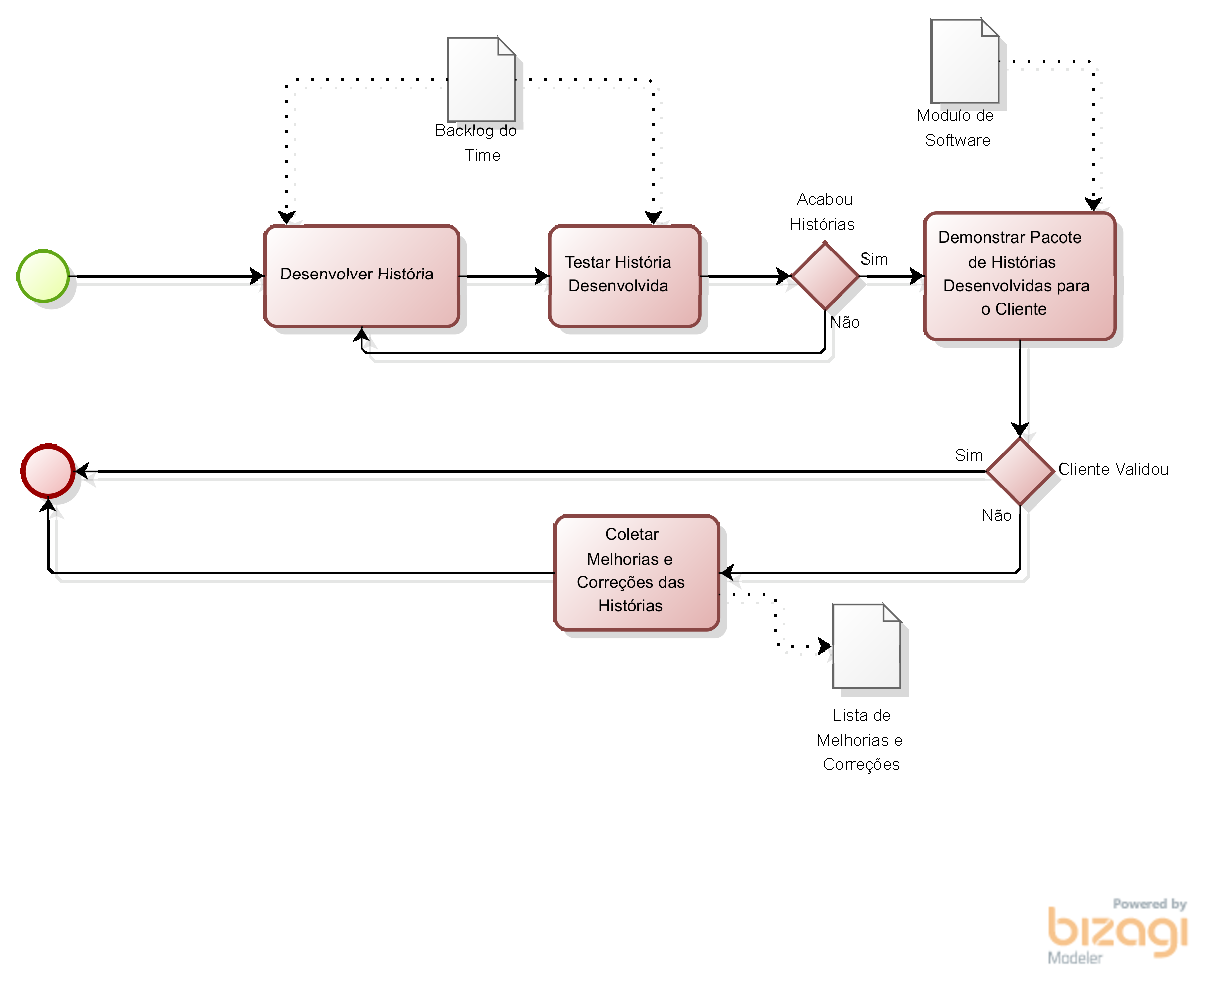
\includegraphics[keepaspectratio=true,scale=0.6]{figuras/desenvolves.eps}
        \caption{Visão geral do sub-processo de desenvolvimento.}
        \label{fig:gerencia}
    \end{figure}

\subsection{Gerência de Mudança}\label{sec:gerencia}

  Este sub-processo é responsável por manter a rastreabilidade e concistência dos requisitos.
  Está presente em todos os nível do processo, uma vez que podem haver mudanças que impactam todos
  os níveis. Por exemplo: Suponha que haja uma mudança durante o desenvolvimento de uma sprint.
  Essa mudança deve ser atualizada no backlog do time, caso essa nova história não esteja mapeada com
  uma feature, deve-se atualizar o backlog do programa e o mesmo para o backlog do portifólio.

\subsubsection{Processo}
  \begin{figure}[H]
      \centering
    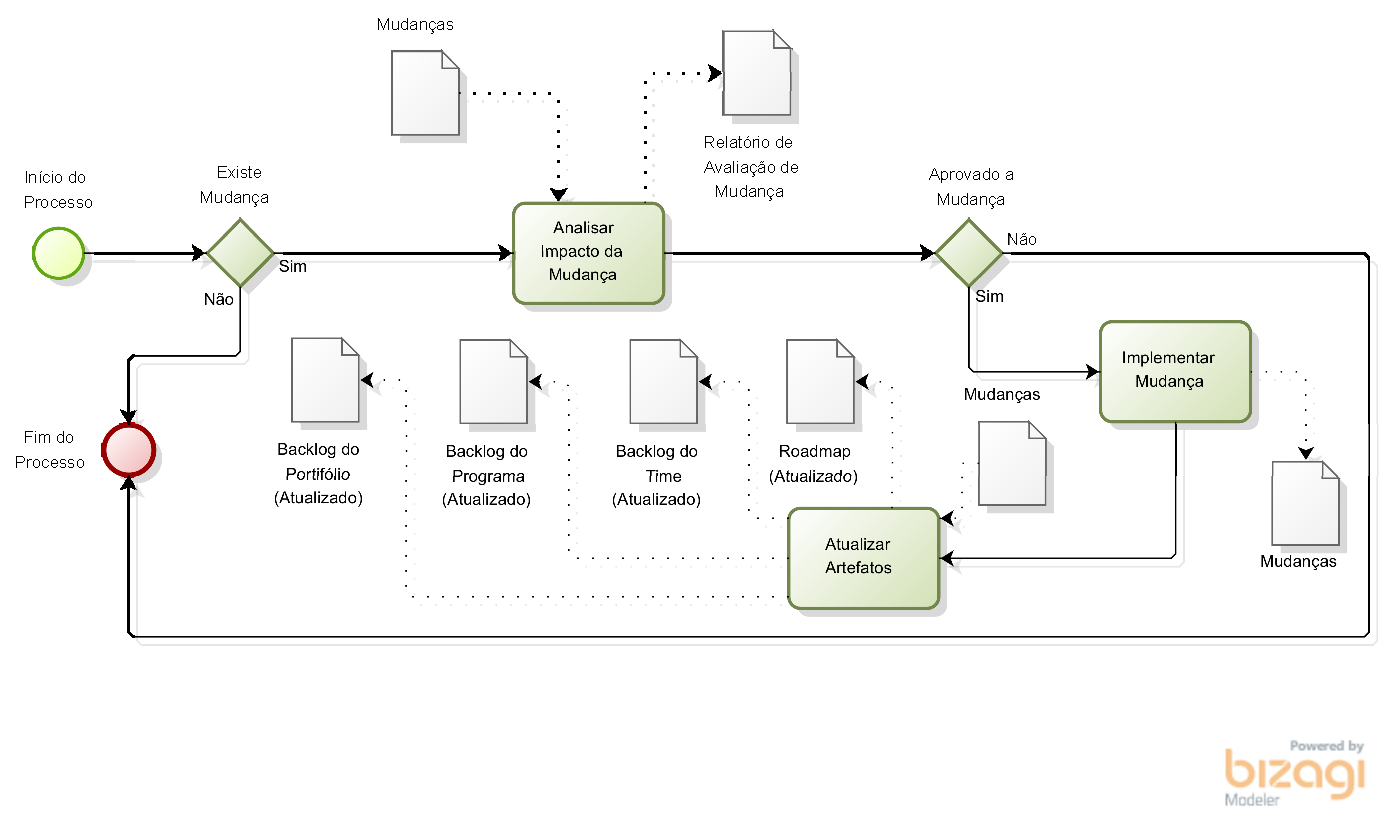
\includegraphics[keepaspectratio=true,scale=0.6]{figuras/gerencia.eps}
      \caption{Visão geral do processo de gerência de mudança.}
      \label{fig:gerencia}
  \end{figure}

\subsubsection{Papéis}

  \textbf{GERENTE DE PORTFÓLIO}: No tratamento de mudanças, não haverá um papel especifico devido
à dimensão do projeto, cabendo a ele a responsabilidade de também gerir mudanças, caso necessário.

\subsubsection{Artefatos}

\begin{description}
  \item[A - Solicitação de Mudança: ]
  Lista com as mudanças que necessitam ser analisadas pela gerência, a lista contém
  uma síntese detalhando porque a mudança foi solicitada.
  \item [B - Mudanças: ] Representa a rastreabilidade dessa mudança, detalhando em
  quais níveis ela irá impactar e qual será o custo para efetivar essa mudança.
  \item [C - Relatório de Avaliação de mundanças: ] O relatório explica o motivo e impactos da aceite
  ou recusa de uma mudança, e serve como base para realização das mudanças.
\end{description}

\subsubsection{Atividades}

\begin{table}[H]
  \centering
    \begin{tabular}{| m{5em} | m{10cm} |}
      \hline
      ID       & 16   \\ \hline
      Nome     & Rastrear Mudanças  \\ \hline
      Objetivo & ---  \\ \hline
      Entradas & Solicitação de Mudança\\ \hline
      Saídas   & Mudanças \\ \hline
      Papel Responsável   & Gerente de Portfólio. \\ \hline
    \end{tabular}
    \caption{Legenda da Tabela}
    \label{tabela:atividade16}
\end{table}

\begin{table}[H]
  \centering
    \begin{tabular}{| m{5em} | m{10cm} |}
      \hline
      ID       & 17   \\ \hline
      Nome     & Analisar Impacto da Mudança \\ \hline
      Objetivo & ---  \\ \hline
      Entradas & Mudanças \\ \hline
      Saídas   & Relatório de Avaliação de Mudança \\ \hline
      Papel Responsável   & Gerente de Portfólio. \\ \hline
    \end{tabular}
    \caption{Legenda da Tabela}
    \label{tabela:atividade17}
\end{table}

\begin{table}[H]
  \centering
    \begin{tabular}{| m{5em} | m{10cm} |}
      \hline
      ID       & 18   \\ \hline
      Nome     & Atualizar Backlog do Time  \\ \hline
      Objetivo & ---  \\ \hline
      Entradas & Mudanças \\ \hline
      Saídas   & Backlog do Time (Atualizado) \\ \hline
      Papel Responsável   & Gerente de Portfólio. \\ \hline
    \end{tabular}
    \caption{Legenda da Tabela}
    \label{tabela:atividade18}
\end{table}

\begin{table}[H]
  \centering
    \begin{tabular}{| m{5em} | m{10cm} |}
      \hline
      ID       & 19   \\ \hline
      Nome     & Atualizar Backlog do Programa  \\ \hline
      Objetivo & ---  \\ \hline
      Entradas & Mudanças\\ \hline
      Saídas   & Backlog do Programa (Atualizado). \\ \hline
      Papel Responsável   & Gerente de Portfólio. \\ \hline
    \end{tabular}
    \caption{Legenda da Tabela}
    \label{tabela:atividade19}
\end{table}

\begin{table}[H]
  \centering
    \begin{tabular}{| m{5em} | m{10cm} |}
      \hline
      ID       & 20   \\ \hline
      Nome     & Atualizar Backlog do Portifólio  \\ \hline
      Objetivo & ---  \\ \hline
      Entradas & Mudanças \\ \hline
      Saídas   & Backlog do Portifólio Atualizado \\ \hline
      Papel Responsável   & Gerente de Portfólio. \\ \hline
    \end{tabular}
    \caption{Legenda da Tabela}
    \label{tabela:atividade20}
\end{table}
